\clearpage
%%__________________________________________________________________||
\section{Results}
\label{sec:interpretation}

A likelihood model of the observations in all data samples is used to
obtain a consistent prediction of the SM backgrounds and to test for
the presence of a variety of signal models.  In each bin of \scalht
for events in the same category of \njet and \nb, the observation is
modelled as a Poisson-distributed variable around the sum of the SM
expectation and a potential signal contribution (assumed to be zero in
the following discussion). The SM expectation is related to the
expected yields in the \mj, \mmj, and \gj control samples via transfer
factors derived from simulation. Likelihood functions describe the
yields in the \scalht bins of the \mj, \mmj, and \gj control samples
in the same category of \njet and \nb as the signal region. The
systematic uncertainties summarised in Table~\ref{tab:bkgd_systs} are
accommodated in the likelihood function by nuisance parameters, the
measurements of which are assumed to follow a log-normal
distribution. In the presence of a non-zero signal contribution, the
CL$_{\mathrm{s}}$ technique~\cite{read, Cowan:2010js} is used to
determine upper limits on production cross section using asymptotic
formulae.

The expected number of events from SM processes is determined from a
simultaneous fit to the signal region and up to three control
samples. The likelihood function is maximised over all fit parameters
under the SM-only hypothesis.
Tables~\ref{tab:predewkdata_sig_comb_mono}--\ref{tab:predewkdata_sig_comb_sym} 
summarise the observed yields and ``a priori'' and ``a posteriori'' SM
expectations for signal candidate events in the monojet, asymmetric,
and symmetric categories, respectively. No significant tension is
observed between the predictions and data in the signal region, which
is well described by the SM-only hypothesis.

\begin{table}[h!]
\scriptsize
\centering
\caption{
  Observed data counts, ``pre-fit'' and ``post-fit'' background expectations  
  for all the \scalht bins and \njet, \nb multiplicity in the monojet event category. 
  The uncertainties include statistical as well as systematic contributions. 
  \label{tab:predewkdata_sig_comb_mono}}  
\scalebox{0.85}{\begin{tabular}{lccccccccc}
	\hline\hline
                    &              & \multicolumn{8}{c}{\scalht (\gev)}                                                                                                                                    \\ 
                    & (\njet, \nb) & 200-250               & 250-300              & 300-350              & 350-400            & 400-500            & 500-600            & 600-800           & 800-$\infty$ \\ [0.8ex] 
\hline
 Data & $(1j,0)$ & $13094$ & $4130$ & $1477$ & $663$ & $461$ & $118$ & $50$ & -- \\[0.5ex]
 SM pre-fit & $(1j,0)$ & $12319.3\pm985.8$ & $4167.9\pm384.1$ & $1474.1\pm155.2$ & $559.8\pm95.2$ & $463.1\pm74.5$ & $145.6\pm29.1$ & $60.4\pm25.1$ & -- \\[0.5ex]
 SM post-fit & $(1j,0)$ & $13012.3\pm112.8$ & $4133.5\pm57.7$ & $1480.8\pm33.9$ & $638.0\pm21.4$ & $439.5\pm16.0$ & $118.1\pm7.0$ & $51.3\pm6.4$ & -- \\[0.5ex]
 Data & $(1j,1)$ & $475$ & $151$ & $57$ & $25$ & $24$ & $6$ & -- & -- \\[0.5ex]
 SM pre-fit & $(1j,1)$ & $505.3\pm64.3$ & $169.6\pm24.6$ & $61.3\pm10.3$ & $21.3\pm4.5$ & $21.0\pm4.4$ & $4.7\pm1.3$ & -- & -- \\[0.5ex]
 SM post-fit & $(1j,1)$ & $488.4\pm18.1$ & $157.9\pm11.0$ & $58.1\pm6.2$ & $24.1\pm3.8$ & $20.8\pm2.6$ & $5.3\pm1.4$ & -- & -- \\[0.5ex]

	\hline
	\hline
\end{tabular}}
\end{table}

\clearpage
\begin{table}[h!]
\scriptsize
\centering
\caption{
  Observed data counts, ``pre-fit'' and ``post-fit'' background expectations  
  for all the \scalht bins and \njet, \nb multiplicity in the asymmetric event category. 
  The uncertainties include statistical as well as systematic contributions. 
  \label{tab:predewkdata_sig_comb_asym}}  
\scalebox{0.85}{\begin{tabular}{lccccccccc}
	\hline\hline
                    &                   & \multicolumn{8}{c}{\scalht (\gev)}                                                                                                                              \\ 
                    & (\njet, \nb)      & 200-250              & 250-300              & 300-350            & 350-400            & 400-500            & 500-600          & 600-800          & 800-$\infty$ \\ [0.8ex] 
\hline

 Data & $(2a,0)$ & $5788$ & $1585$ & $584$ & $232$ & $139$ & $26$ & $16$ & -- \\[0.5ex]
 SM pre-fit & $(2a,0)$ & $5890.6\pm544.0$ & $1695.0\pm180.5$ & $601.3\pm65.1$ & $224.3\pm38.4$ & $144.4\pm25.0$ & $36.4\pm7.1$ & $21.0\pm8.1$ & -- \\[0.5ex]
 SM post-fit & $(2a,0)$ & $5831.5\pm81.6$ & $1621.6\pm35.0$ & $581.0\pm17.9$ & $227.5\pm9.5$ & $136.5\pm6.4$ & $30.0\pm2.6$ & $18.3\pm3.2$ & -- \\[0.5ex]
 Data & $(2a,1)$ & $536$ & $152$ & $51$ & $18$ & $7$ & $4$ & -- & -- \\[0.5ex]
 SM pre-fit & $(2a,1)$ & $543.8\pm62.0$ & $161.7\pm22.6$ & $49.3\pm7.7$ & $20.5\pm3.9$ & $12.9\pm2.6$ & $4.3\pm1.0$ & -- & -- \\[0.5ex]
 SM post-fit & $(2a,1)$ & $541.0\pm16.4$ & $153.8\pm7.1$ & $49.7\pm3.7$ & $19.7\pm2.2$ & $10.7\pm1.4$ & $4.0\pm1.0$ & -- & -- \\[0.5ex]
 Data & $(2a,2)$ & $31$ & $10$ & $3$ & $1$ & $0$ & -- & -- & -- \\[0.5ex]
 SM pre-fit & $(2a,2)$ & $29.7\pm4.0$ & $7.2\pm1.2$ & $6.5\pm1.2$ & $2.0\pm0.5$ & $0.8\pm0.2$ & -- & -- & -- \\[0.5ex]
 SM post-fit & $(2a,2)$ & $29.5\pm3.5$ & $7.4\pm1.2$ & $5.0\pm1.1$ & $1.8\pm0.6$ & $0.6\pm0.3$ & -- & -- & -- \\[0.5ex]
 Data & $(3a,0)$ & $1599$ & $1609$ & $777$ & $239$ & $95$ & $15$ & $9$ & -- \\[0.5ex]
 SM pre-fit & $(3a,0)$ & $1669.4\pm163.3$ & $1529.4\pm171.2$ & $822.9\pm127.9$ & $272.3\pm60.5$ & $111.3\pm18.2$ & $19.7\pm4.0$ & $9.3\pm4.1$ & -- \\[0.5ex]
 SM post-fit & $(3a,0)$ & $1624.8\pm39.6$ & $1561.5\pm44.5$ & $781.7\pm28.8$ & $258.7\pm13.4$ & $100.9\pm5.4$ & $16.5\pm1.7$ & $8.0\pm1.5$ & -- \\[0.5ex]
 Data & $(3a,1)$ & $340$ & $299$ & $152$ & $59$ & $15$ & $1$ & $1$ & -- \\[0.5ex]
 SM pre-fit & $(3a,1)$ & $340.3\pm38.6$ & $357.2\pm51.6$ & $156.6\pm28.2$ & $46.1\pm12.0$ & $14.6\pm2.7$ & $2.3\pm0.7$ & $1.1\pm0.5$ & -- \\[0.5ex]
 SM post-fit & $(3a,1)$ & $340.7\pm12.6$ & $335.8\pm13.1$ & $148.6\pm7.9$ & $47.1\pm3.6$ & $13.0\pm1.4$ & $2.0\pm0.5$ & $1.0\pm0.4$ & -- \\[0.5ex]
 Data & $(3a,2)$ & $52$ & $62$ & $29$ & $12$ & $1$ & $0$ & -- & -- \\[0.5ex]
 SM pre-fit & $(3a,2)$ & $59.3\pm7.6$ & $61.9\pm10.1$ & $34.2\pm7.0$ & $11.2\pm3.2$ & $1.9\pm0.4$ & $0.4\pm0.1$ & -- & -- \\[0.5ex]
 SM post-fit & $(3a,2)$ & $58.3\pm4.6$ & $60.1\pm3.8$ & $31.3\pm2.7$ & $11.1\pm1.5$ & $1.5\pm0.4$ & $0.4\pm0.2$ & -- & -- \\[0.5ex]
 Data & $(3a,\geq 3)$ & $3$ & $1$ & $1$ & -- & -- & -- & -- & -- \\[0.5ex]
 SM pre-fit & $(3a,\geq 3)$ & $0.9\pm0.2$ & $1.9\pm0.4$ & $0.8\pm0.2$ & -- & -- & -- & -- & -- \\[0.5ex]
 SM post-fit & $(3a,\geq 3)$ & $1.3\pm0.5$ & $1.5\pm0.6$ & $0.8\pm0.4$ & -- & -- & -- & -- & -- \\[0.5ex]
 Data & $(4a,0)$ & $3$ & $178$ & $412$ & $246$ & $119$ & $15$ & $2$ & -- \\[0.5ex]
 SM pre-fit & $(4a,0)$ & $3.8\pm0.5$ & $153.4\pm18.5$ & $462.8\pm89.5$ & $285.1\pm64.1$ & $142.4\pm22.6$ & $14.7\pm3.2$ & $2.6\pm1.2$ & -- \\[0.5ex]
 SM post-fit & $(4a,0)$ & $4.1\pm1.0$ & $159.3\pm10.8$ & $418.0\pm19.5$ & $256.7\pm14.2$ & $128.0\pm7.6$ & $12.9\pm1.7$ & $2.2\pm0.6$ & -- \\[0.5ex]
 Data & $(4a,1)$ & $1$ & $53$ & $180$ & $96$ & $51$ & $4$ & $0$ & -- \\[0.5ex]
 SM pre-fit & $(4a,1)$ & $1.4\pm0.3$ & $51.5\pm7.5$ & $189.7\pm39.6$ & $108.1\pm25.9$ & $55.6\pm10.1$ & $3.1\pm0.8$ & $0.6\pm0.3$ & -- \\[0.5ex]
 SM post-fit & $(4a,1)$ & $1.6\pm0.5$ & $50.7\pm4.6$ & $172.6\pm9.2$ & $98.9\pm6.8$ & $49.0\pm3.9$ & $2.9\pm0.6$ & $0.5\pm0.1$ & -- \\[0.5ex]
 Data & $(4a,2)$ & $0$ & $11$ & $44$ & $30$ & $8$ & $0$ & $0$ & -- \\[0.5ex]
 SM pre-fit & $(4a,2)$ & $0.3\pm0.1$ & $14.6\pm2.4$ & $58.5\pm12.8$ & $30.0\pm7.8$ & $15.6\pm3.3$ & $0.6\pm0.2$ & $0.1\pm0.1$ & -- \\[0.5ex]
 SM post-fit & $(4a,2)$ & $0.3\pm0.2$ & $13.9\pm1.5$ & $51.6\pm4.3$ & $28.7\pm2.9$ & $12.7\pm1.6$ & $0.6\pm0.2$ & $0.1\pm0.0$ & -- \\[0.5ex]
 Data & $(4a,\geq 3)$ & -- & $0$ & $0$ & $2$ & $2$ & -- & -- & -- \\[0.5ex]
 SM pre-fit & $(4a,\geq 3)$ & -- & $1.8\pm0.4$ & $3.2\pm0.8$ & $2.8\pm0.8$ & $1.9\pm0.5$ & -- & -- & -- \\[0.5ex]
 SM post-fit & $(4a,\geq 3)$ & -- & $1.3\pm0.5$ & $2.4\pm0.8$ & $2.3\pm0.7$ & $2.1\pm0.6$ & -- & -- & -- \\[0.5ex]
 Data & $(\geq 5a,0)$ & -- & $3$ & $40$ & $96$ & $105$ & $20$ & $3$ & -- \\[0.5ex]
 SM pre-fit & $(\geq 5a,0)$ & -- & $3.9\pm1.1$ & $49.2\pm8.4$ & $137.6\pm40.4$ & $138.2\pm25.5$ & $22.0\pm5.1$ & $4.5\pm2.0$ & -- \\[0.5ex]
 SM post-fit & $(\geq 5a,0)$ & -- & $2.9\pm1.3$ & $43.5\pm4.7$ & $107.8\pm8.9$ & $114.4\pm8.6$ & $19.6\pm2.6$ & $3.3\pm0.9$ & -- \\[0.5ex]
 Data & $(\geq 5a,1)$ & -- & $0$ & $24$ & $60$ & $74$ & $15$ & $0$ & -- \\[0.5ex]
 SM pre-fit & $(\geq 5a,1)$ & -- & $1.2\pm0.4$ & $22.0\pm3.9$ & $64.5\pm20.4$ & $80.0\pm16.7$ & $17.9\pm4.8$ & $1.9\pm0.9$ & -- \\[0.5ex]
 SM post-fit & $(\geq 5a,1)$ & -- & $0.8\pm0.5$ & $22.2\pm3.0$ & $57.4\pm5.9$ & $71.9\pm5.7$ & $15.4\pm2.3$ & $1.4\pm0.5$ & -- \\[0.5ex]
 Data & $(\geq 5a,2)$ & -- & $0$ & $11$ & $27$ & $29$ & $6$ & $1$ & -- \\[0.5ex]
 SM pre-fit & $(\geq 5a,2)$ & -- & $0.0\pm0.0$ & $6.8\pm1.3$ & $31.7\pm9.8$ & $32.1\pm7.1$ & $6.3\pm1.9$ & $0.5\pm0.3$ & -- \\[0.5ex]
 SM post-fit & $(\geq 5a,2)$ & -- & $0.0\pm0.0$ & $7.9\pm1.7$ & $27.3\pm3.3$ & $28.9\pm3.3$ & $5.5\pm1.2$ & $0.4\pm0.2$ & -- \\[0.5ex]
 Data & $(\geq 5a,\geq 3)$ & -- & -- & $0$ & $2$ & $5$ & $1$ & -- & -- \\[0.5ex]
 SM pre-fit & $(\geq 5a,\geq 3)$ & -- & -- & $0.5\pm0.1$ & $3.6\pm1.1$ & $5.0\pm1.3$ & $0.8\pm0.3$ & -- & -- \\[0.5ex]
 SM post-fit & $(\geq 5a,\geq 3)$ & -- & -- & $0.5\pm0.3$ & $3.0\pm0.9$ & $4.5\pm1.1$ & $0.9\pm0.4$ & -- & -- \\[0.5ex]



	\hline
	\hline
\end{tabular}}
\end{table}

\clearpage
{\begin{table}[h!]
\scriptsize
\centering
\caption{%CMS {\it Preliminary}, $\mathcal{L}_{\mathrm{int}} =
  %2.2\fbinv$, $\sqrt{s} = 13\TeV$. 
  %\newline
  Observed data counts and ``post-fit'' background expectations  
  based on the result of a combined fit to the signal region and multiple
  control regions under the SM-only hypothesis for the ``symmetric''
  event categories. The rows labelled SM ``pre-fit'' show the
  background expectations when excluding the signal region from the
  fit. The uncertainties include statistical as well as systematic
  contributions. 
  \label{tab:predewkdata_sig_comb_sym}}  
\scalebox{0.85}{\begin{tabular}{lccccccccc}
    \hline\hline
                &                  & \multicolumn{8}{c}{\scalht (\gev)}                                                                                                                                    \\ 
                & (\njet, \nb)     & 200-250             & 250-300             & 300-350            & 350-400            & 400-500            & 500-600            & 600-800           & 800-$\infty$      \\ [0.8ex] 
    \hline
    Data        & (2, 0)           & 968                 & 997                 & 657                & 398                & 301                & 110                & 56                & 49                \\[0.5ex] 
    SM post-fit & (2, 0)           & $969.9\pm{ 51.2 }$  & $996.4\pm{ 36.2 }$  & $656.8\pm{ 25.1 }$ & $395.5\pm{ 18.7 }$ & $312.3\pm{ 16.4 }$ & $107.3\pm{ 10.6 }$ & $53.1\pm{ 6.2 }$  & $47.2\pm{ 6.4 }$  \\[0.5ex] 
    SM pre-fit  & (2, 0)           & $943.9\pm{ 134.2 }$ & $938.4\pm{ 148.4 }$ & $627.9\pm{ 86.0 }$ & $341.4\pm{ 61.3 }$ & $329.1\pm{ 38.4 }$ & $105.2\pm{ 24.3 }$ & $43.8\pm{ 12.2 }$ & $44.4\pm{ 11.4 }$ \\[0.5ex] 
    Data        & (2, 1)           & 111                 & 100                 & 65                 & 37                 & 35                 & 5                  & 4                 & 2                 \\[0.5ex] 
    SM post-fit & (2, 1)           & $104.2\pm{ 9.5 }$   & $87.1\pm{ 8.1 }$    & $54.9\pm{ 6.0 }$   & $33.4\pm{ 4.4 }$   & $26.4\pm{ 2.8 }$   & $8.1\pm{ 1.6 }$    & $4.2\pm{ 1.2 }$   & $3.4\pm{ 0.9 }$   \\[0.5ex] 
    SM pre-fit  & (2, 1)           & $80.9\pm{ 16.0 }$   & $57.9\pm{ 11.1 }$   & $40.8\pm{ 7.3 }$   & $26.8\pm{ 5.7 }$   & $24.1\pm{ 3.7 }$   & $9.5\pm{ 2.7 }$    & $4.0\pm{ 1.4 }$   & $3.7\pm{ 1.3 }$   \\[0.5ex] 
    Data        & (2, 2)           & 7                   & 4                   & 2                  & 3                  & 3                  & 0                  & 0                 & --                \\[0.5ex] 
    SM post-fit & (2, 2)           & $4.6\pm{ 1.8 }$     & $2.7\pm{ 1.2 }$     & $3.0\pm{ 1.3 }$    & $1.5\pm{ 0.7 }$    & $1.4\pm{ 0.4 }$    & $1.0\pm{ 0.5 }$    & $0.2\pm{ 0.2 }$   & --                \\[0.5ex] 
    SM pre-fit  & (2, 2)           & $1.1\pm{ 2.3 }$     & $0.8\pm{ 1.9 }$     & $3.4\pm{ 2.0 }$    & $0.7\pm{ 0.8 }$    & $1.1\pm{ 0.5 }$    & $1.3\pm{ 0.8 }$    & $0.2\pm{ 0.2 }$   & --                \\[0.5ex] 
    Data        & (3, 0)           & 2                   & 176                 & 505                & 491                & 547                & 185                & 90                & 72                \\[0.5ex] 
    SM post-fit & (3, 0)           & $1.4\pm{ 1.4 }$     & $175.8\pm{ 13.3 }$  & $504.3\pm{ 26.5 }$ & $484.8\pm{ 20.5 }$ & $541.3\pm{ 24.0 }$ & $189.0\pm{ 15.3 }$ & $89.9\pm{ 8.2 }$  & $71.0\pm{ 7.2 }$  \\[0.5ex] 
    SM pre-fit  & (3, 0)           & $0.0\pm{ 2.4 }$     & $173.6\pm{ 26.2 }$  & $491.8\pm{ 63.6 }$ & $421.9\pm{ 58.6 }$ & $499.2\pm{ 65.1 }$ & $195.4\pm{ 36.8 }$ & $89.5\pm{ 23.7 }$ & $68.0\pm{ 11.6 }$ \\[0.5ex] 
    Data        & (3, 1)           & --                  & 38                  & 90                 & 100                & 76                 & 30                 & 15                & 10                \\[0.5ex] 
    SM post-fit & (3, 1)           & --                  & $38.1\pm{ 4.1 }$    & $82.0\pm{ 7.4 }$   & $93.7\pm{ 7.0 }$   & $79.3\pm{ 6.8 }$   & $27.3\pm{ 3.6 }$   & $15.2\pm{ 2.8 }$  & $9.6\pm{ 1.6 }$   \\[0.5ex] 
    SM pre-fit  & (3, 1)           & --                  & $37.9\pm{ 6.3 }$    & $70.5\pm{ 11.1 }$  & $81.2\pm{ 11.9 }$  & $79.2\pm{ 11.6 }$  & $26.4\pm{ 5.9 }$   & $15.3\pm{ 4.1 }$  & $9.2\pm{ 2.0 }$   \\[0.5ex] 
    Data        & (3, 2)           & --                  & 10                  & 10                 & 10                 & 13                 & 5                  & 1                 & 1                 \\[0.5ex] 
    SM post-fit & (3, 2)           & --                  & $6.9\pm{ 1.5 }$     & $15.3\pm{ 2.3 }$   & $15.8\pm{ 2.1 }$   & $12.0\pm{ 1.8 }$   & $3.6\pm{ 0.7 }$    & $0.8\pm{ 0.3 }$   & $1.0\pm{ 0.3 }$   \\[0.5ex] 
    SM pre-fit  & (3, 2)           & --                  & $5.9\pm{ 1.7 }$     & $17.5\pm{ 3.2 }$   & $16.4\pm{ 3.0 }$   & $11.3\pm{ 2.2 }$   & $3.4\pm{ 1.0 }$    & $0.8\pm{ 0.3 }$   & $0.9\pm{ 0.3 }$   \\[0.5ex] 
    Data        & (3, $\ge3$)      & --                  & 0                   & --                 & --                 & 1                  & --                 & --                & --                \\[0.5ex] 
    SM post-fit & (3, $\ge3$)      & --                  & $0.1\pm{ 0.2 }$     & --                 & --                 & $0.5\pm{ 0.2 }$    & --                 & --                & --                \\[0.5ex] 
    SM pre-fit  & (3, $\ge3$)      & --                  & $0.0\pm{ 0.3 }$     & --                 & --                 & $0.4\pm{ 0.2 }$    & --                 & --                & --                \\[0.5ex] 
    Data        & (4, 0)           & --                  & --                  & 60                 & 148                & 308                & 157                & 104               & 60                \\[0.5ex] 
    SM post-fit & (4, 0)           & --                  & --                  & $57.4\pm{ 7.5 }$   & $149.5\pm{ 14.3 }$ & $309.1\pm{ 16.5 }$ & $156.9\pm{ 12.4 }$ & $102.2\pm{ 9.6 }$ & $56.6\pm{ 6.2 }$  \\[0.5ex] 
    SM pre-fit  & (4, 0)           & --                  & --                  & $48.8\pm{ 14.1 }$  & $163.1\pm{ 65.7 }$ & $301.0\pm{ 46.9 }$ & $155.8\pm{ 36.3 }$ & $96.5\pm{ 19.1 }$ & $52.8\pm{ 11.3 }$ \\[0.5ex] 
    Data        & (4, 1)           & --                  & --                  & 12                 & 72                 & 101                & 31                 & 15                & 9                 \\[0.5ex] 
    SM post-fit & (4, 1)           & --                  & --                  & $15.3\pm{ 2.7 }$   & $71.5\pm{ 8.5 }$   & $94.5\pm{ 7.6 }$   & $34.2\pm{ 4.3 }$   & $18.1\pm{ 2.6 }$  & $11.3\pm{ 1.8 }$  \\[0.5ex] 
    SM pre-fit  & (4, 1)           & --                  & --                  & $19.9\pm{ 6.3 }$   & $67.1\pm{ 19.0 }$  & $84.6\pm{ 11.7 }$  & $36.9\pm{ 8.3 }$   & $18.4\pm{ 4.3 }$  & $11.6\pm{ 2.5 }$  \\[0.5ex] 
    Data        & (4, 2)           & --                  & --                  & 6                  & 24                 & 34                 & 11                 & 6                 & 2                 \\[0.5ex] 
    SM post-fit & (4, 2)           & --                  & --                  & $4.6\pm{ 1.5 }$    & $21.6\pm{ 3.8 }$   & $33.5\pm{ 3.8 }$   & $8.1\pm{ 1.6 }$    & $3.1\pm{ 0.6 }$   & $2.1\pm{ 0.5 }$   \\[0.5ex] 
    SM pre-fit  & (4, 2)           & --                  & --                  & $3.6\pm{ 2.0 }$    & $17.2\pm{ 5.8 }$   & $31.9\pm{ 5.0 }$   & $7.3\pm{ 2.1 }$    & $2.8\pm{ 0.7 }$   & $2.1\pm{ 0.6 }$   \\[0.5ex] 
    Data        & (4, $\ge3$)      & --                  & --                  & 0                  & 3                  & 0                  & 1                  & 0                 & 0                 \\[0.5ex] 
    SM post-fit & (4, $\ge3$)      & --                  & --                  & $0.2\pm{ 0.3 }$    & $2.1\pm{ 0.9 }$    & $1.2\pm{ 0.6 }$    & $0.7\pm{ 0.3 }$    & $0.1\pm{ 0.1 }$   & $0.1\pm{ 0.0 }$   \\[0.5ex] 
    SM pre-fit  & (4, $\ge3$)      & --                  & --                  & $0.0\pm{ 0.4 }$    & $1.5\pm{ 1.1 }$    & $1.5\pm{ 0.8 }$    & $0.6\pm{ 0.4 }$    & $0.0\pm{ 0.1 }$   & $0.0\pm{ 0.0 }$   \\[0.5ex] 
    Data        & ($\ge5$, 0)      & --                  & --                  & --                 & 7                  & 89                 & 84                 & 75                & 59                \\[0.5ex] 
    SM post-fit & ($\ge5$, 0)      & --                  & --                  & --                 & $10.3\pm{ 2.6 }$   & $88.1\pm{ 9.1 }$   & $81.3\pm{ 8.2 }$   & $74.4\pm{ 7.0 }$  & $58.3\pm{ 6.6 }$  \\[0.5ex] 
    SM pre-fit  & ($\ge5$, 0)      & --                  & --                  & --                 & $15.3\pm{ 5.9 }$   & $86.1\pm{ 13.1 }$  & $78.1\pm{ 20.0 }$  & $71.0\pm{ 14.4 }$ & $46.2\pm{ 12.8 }$ \\[0.5ex] 
    Data        & ($\ge5$, 1)      & --                  & --                  & --                 & 4                  & 42                 & 39                 & 31                & 21                \\[0.5ex] 
    SM post-fit & ($\ge5$, 1)      & --                  & --                  & --                 & $3.0\pm{ 1.0 }$    & $43.3\pm{ 5.0 }$   & $38.9\pm{ 4.6 }$   & $27.8\pm{ 3.2 }$  & $20.0\pm{ 3.3 }$  \\[0.5ex] 
    SM pre-fit  & ($\ge5$, 1)      & --                  & --                  & --                 & $2.5\pm{ 1.5 }$    & $44.1\pm{ 8.0 }$   & $38.9\pm{ 8.7 }$   & $25.3\pm{ 5.6 }$  & $15.8\pm{ 3.5 }$  \\[0.5ex] 
    Data        & ($\ge5$, 2)      & --                  & --                  & --                 & 0                  & 22                 & 12                 & 7                 & 12                \\[0.5ex] 
    SM post-fit & ($\ge5$, 2)      & --                  & --                  & --                 & $1.4\pm{ 0.8 }$    & $20.1\pm{ 3.2 }$   & $14.6\pm{ 2.3 }$   & $7.7\pm{ 1.2 }$   & $6.6\pm{ 1.3 }$   \\[0.5ex] 
    SM pre-fit  & ($\ge5$, 2)      & --                  & --                  & --                 & $2.1\pm{ 1.3 }$    & $18.8\pm{ 4.1 }$   & $15.4\pm{ 3.8 }$   & $7.6\pm{ 1.9 }$   & $4.6\pm{ 1.2 }$   \\[0.5ex] 
    Data        & ($\ge5$, $\ge3$) & --                  & --                  & --                 & --                 & 0                  & 1                  & 0                 & 3                 \\[0.5ex] 
    SM post-fit & ($\ge5$, $\ge3$) & --                  & --                  & --                 & --                 & $0.7\pm{ 0.5 }$    & $1.2\pm{ 0.5 }$    & $1.3\pm{ 0.4 }$   & $1.1\pm{ 0.4 }$   \\[0.5ex] 
    SM pre-fit  & ($\ge5$, $\ge3$) & --                  & --                  & --                 & --                 & $0.7\pm{ 0.7 }$    & $1.2\pm{ 0.7 }$    & $1.4\pm{ 0.5 }$   & $0.8\pm{ 0.3 }$   \\[0.5ex] 
    \hline
    \hline
\end{tabular}}
\end{table}

\clearpage

%%__________________________________________________________________||
\section{Interpretation}

The results of this search are interpreted in terms of upper limits in
the production cross section as a function of the parent sparticle and
LSP mass for simplified models~\cite{Alwall:2008ag, Alwall:2008va,
  sms} that represent the pair production of gluinos and their
subsequent decays to four quarks and two LSPs. The event samples for
the simplified models are generated with \MADGRAPH V5~\cite{madgraph}.
Inclusive, process-dependent, NLO calculations of SUSY production
cross sections, with next-to-leading-logarithmic (NLL) corrections,
are obtained with the program \PROSPINO~\cite{Beenakker:1996ch,
  PhysRevD.80.095004,PhysRevLett.102.111802, PhysRevD.80.095004,
  1126-6708-2009-12-041, doi:10.1142/S0217751X11053560,
  susy-nlo-nll}. The samples are generated using the
CTEQ6L1~\cite{Pumplin:2002vw} PDFs. The distribution of the number of
pp interactions per bunch crossing for the simulated samples matches
that observed in data. Various uncertainties in the experimental
acceptance are considered, for which typical magnitudes are summarised
in Table~\ref{tab:signal_systs}.

\begin{table}[h!]
  \caption{%CMS {\it Simulation}. 
    Typical magnitudes of systematic uncertainties in the experimental
    acceptance for the signal models considered.
  }
  \label{tab:signal_systs}
  \centering
  \footnotesize
  \begin{tabular}{ lccc }
    \hline
    \hline
    Systematic source              & Type          & Correlated & Typical magnitude (\%) \\
    \hline
    Luminosity                     & Normalisation & Yes        & 4.6                    \\
    Monte Carlo statistics         & Norm. + shape & No         & 1--50                  \\
    Initial state radiation        & Norm. + shape & Yes        & 0--30                  \\
    Jet energy scale               & Norm. + shape & Yes        & 3--10                  \\
    Pile-up                        & Norm. + shape & Yes        & 0-5                    \\
    Trigger                        & Norm. + shape & Yes        & 0--10                  \\
    Parton density functions       & Normalisation & No         & 10                     \\
%    Renormalisation/factorisation & Norm. + shape & No         & 10                     \\
    b-tag scale factors            & Norm. + shape & Yes        & 5--30                  \\
    Lepton scale factors           & Normalisation & Yes        & $<$5                   \\
    \hline
    \hline
  \end{tabular}
\end{table}

Figure~\ref{fig:mht-templates} shows for two categories in \njet and
\nb at high \scalht that are expected to provide good sensitivity to
gluino models the distribution of the data observations as a function
of the \mht variable, the expected distribution for the sum of all SM
background processes, and the expected distribution for an example
benchmark signal model.

\begin{figure*}[tbhp]
  \begin{center}
    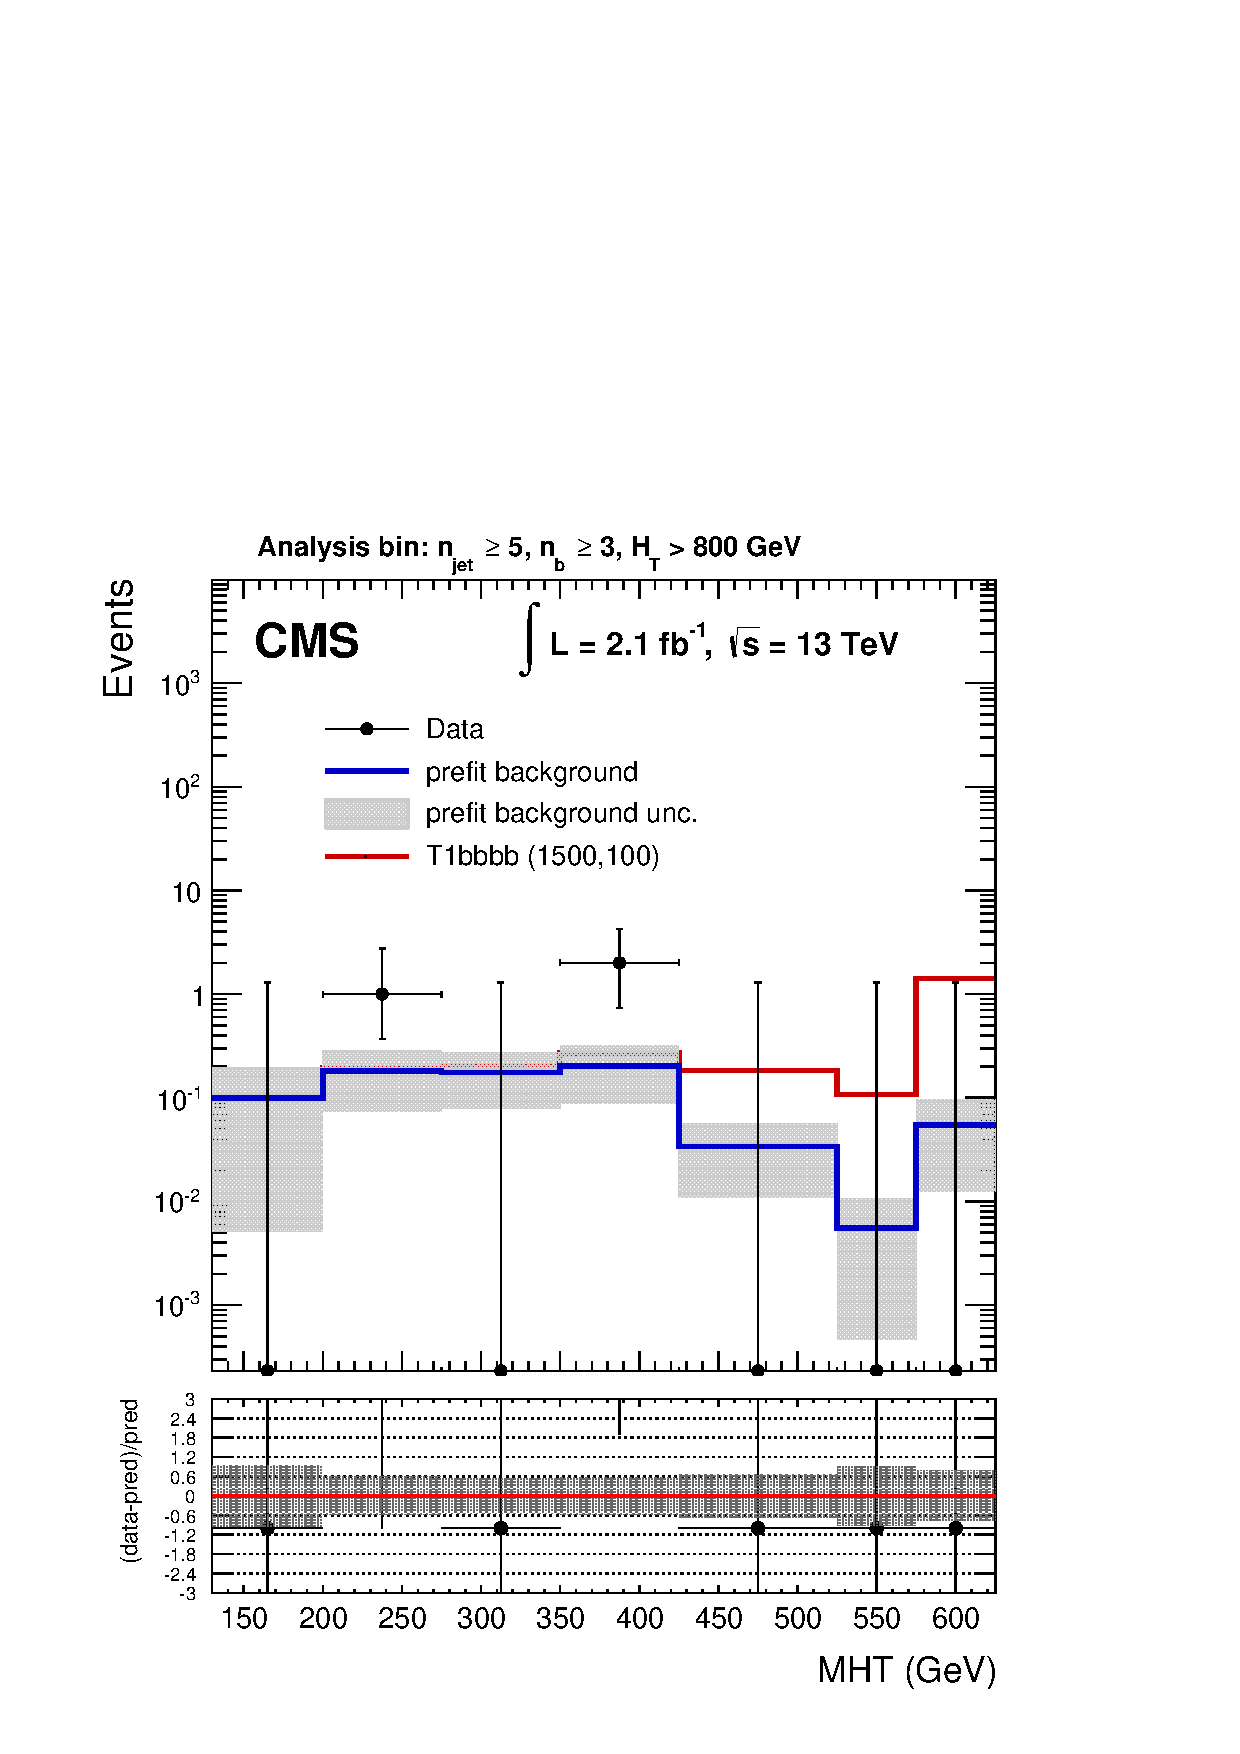
\includegraphics[width=0.5\textwidth]{postFitShape_ge3b_ge5j_800_Inf_prefit} \\
    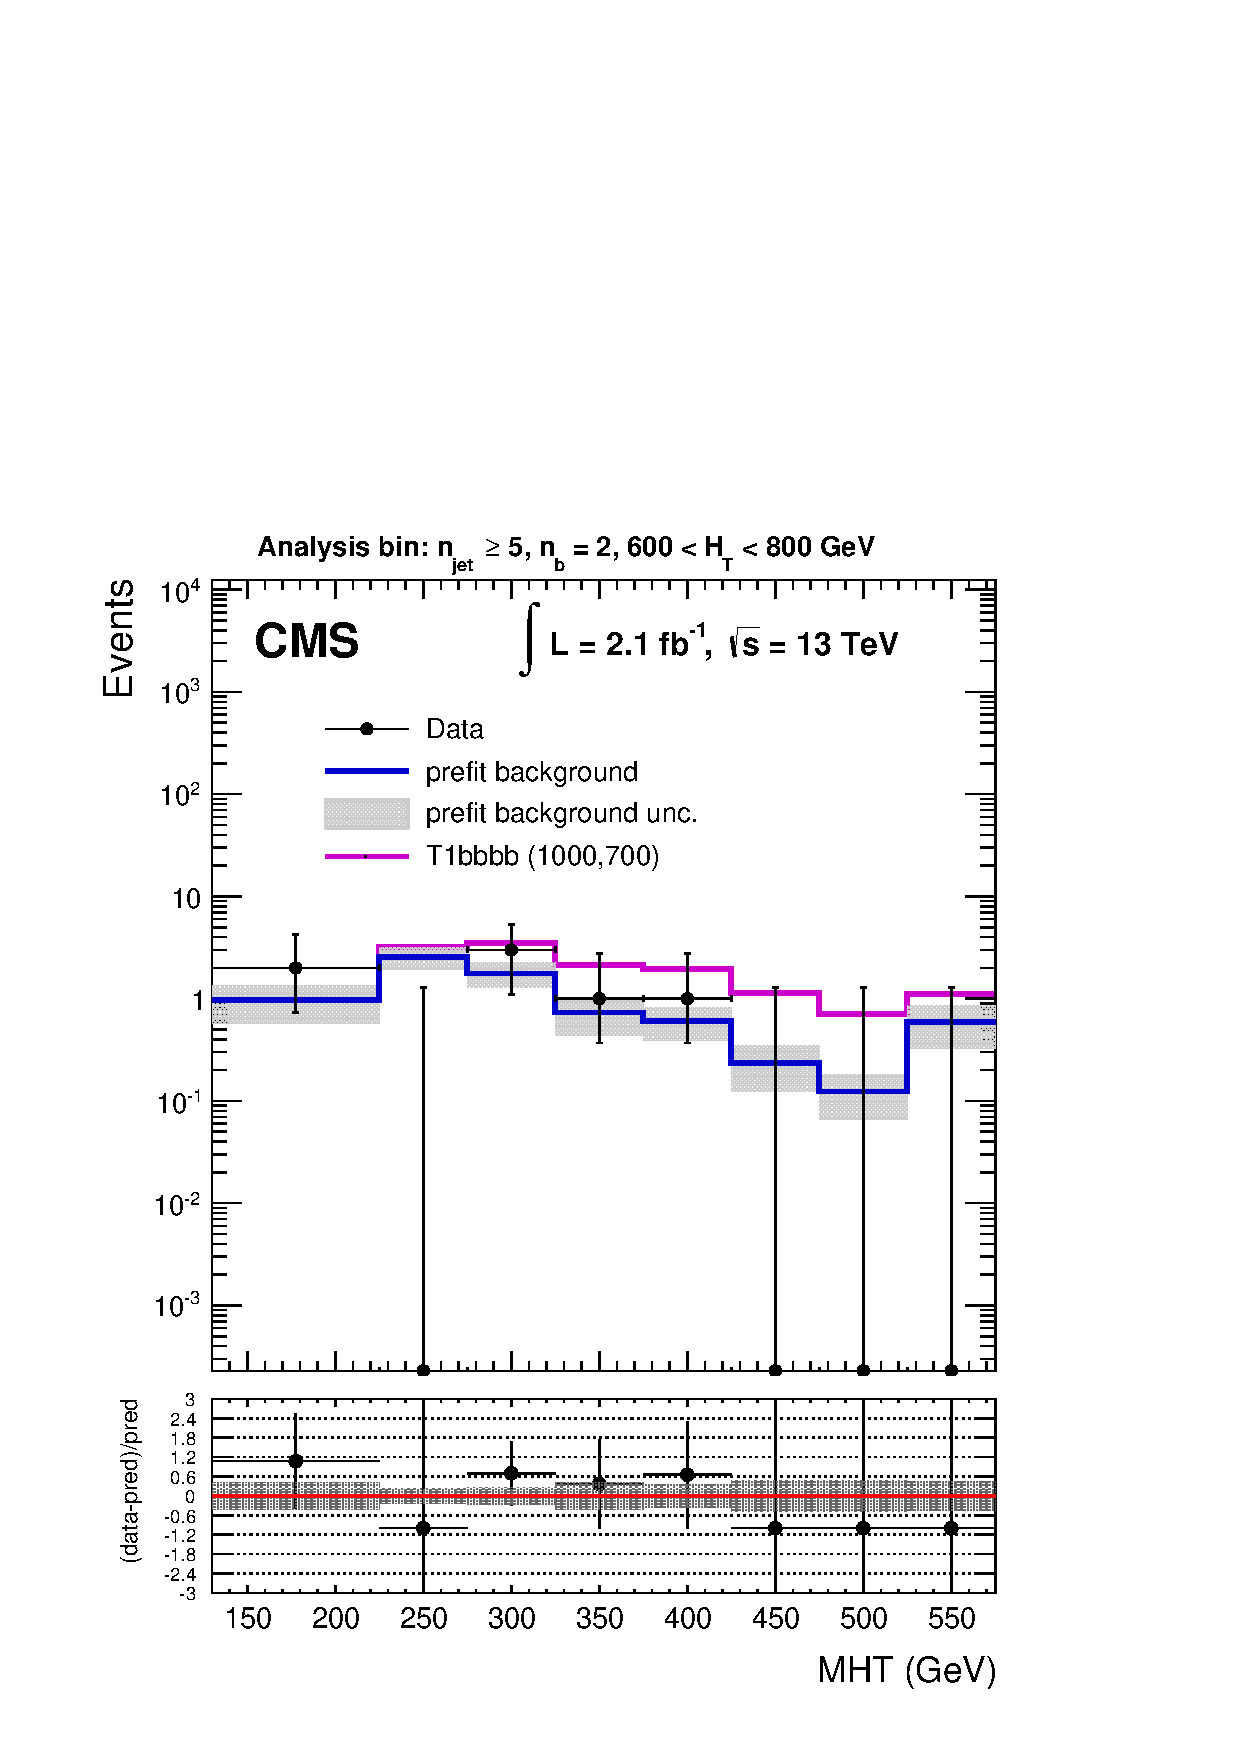
\includegraphics[width=0.5\textwidth]{postFitShape_eq2b_ge5j_600_800_prefit} \\
  \end{center}
  \caption{ The \mht distribution observed in data and the expected
    distribution for the sum of all SM background processes in two
    representative event categories at high \scalht. The expected
    distribution for an example benchmark models with a large (small)
    mass splitting between the gluino and LSP is also shown in the top
    (bottom) figure. \label{fig:mht-templates} }
\end{figure*}
  
\begin{figure*}[thp!]
  \begin{center}
    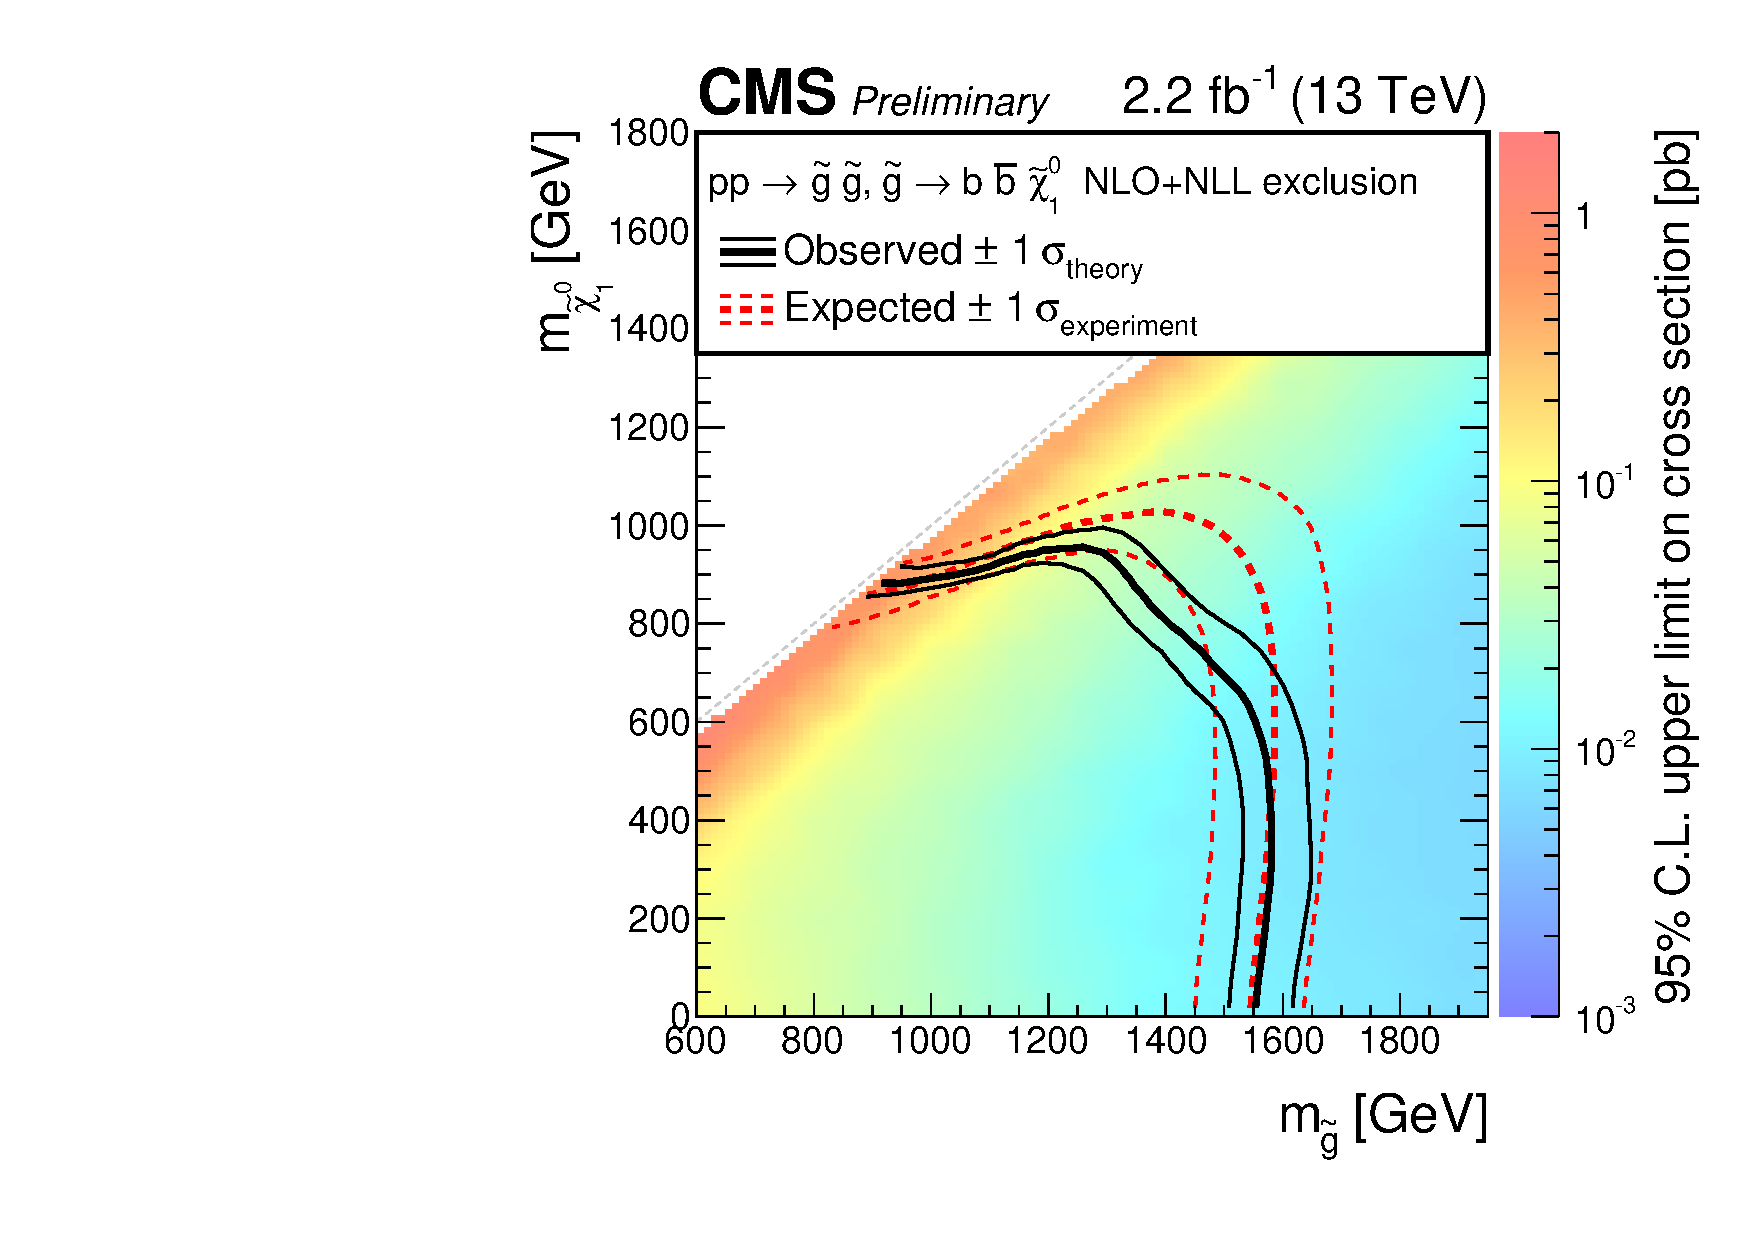
\includegraphics[width=0.65\textwidth]{t1bbbbRA1XSEC.pdf} 
    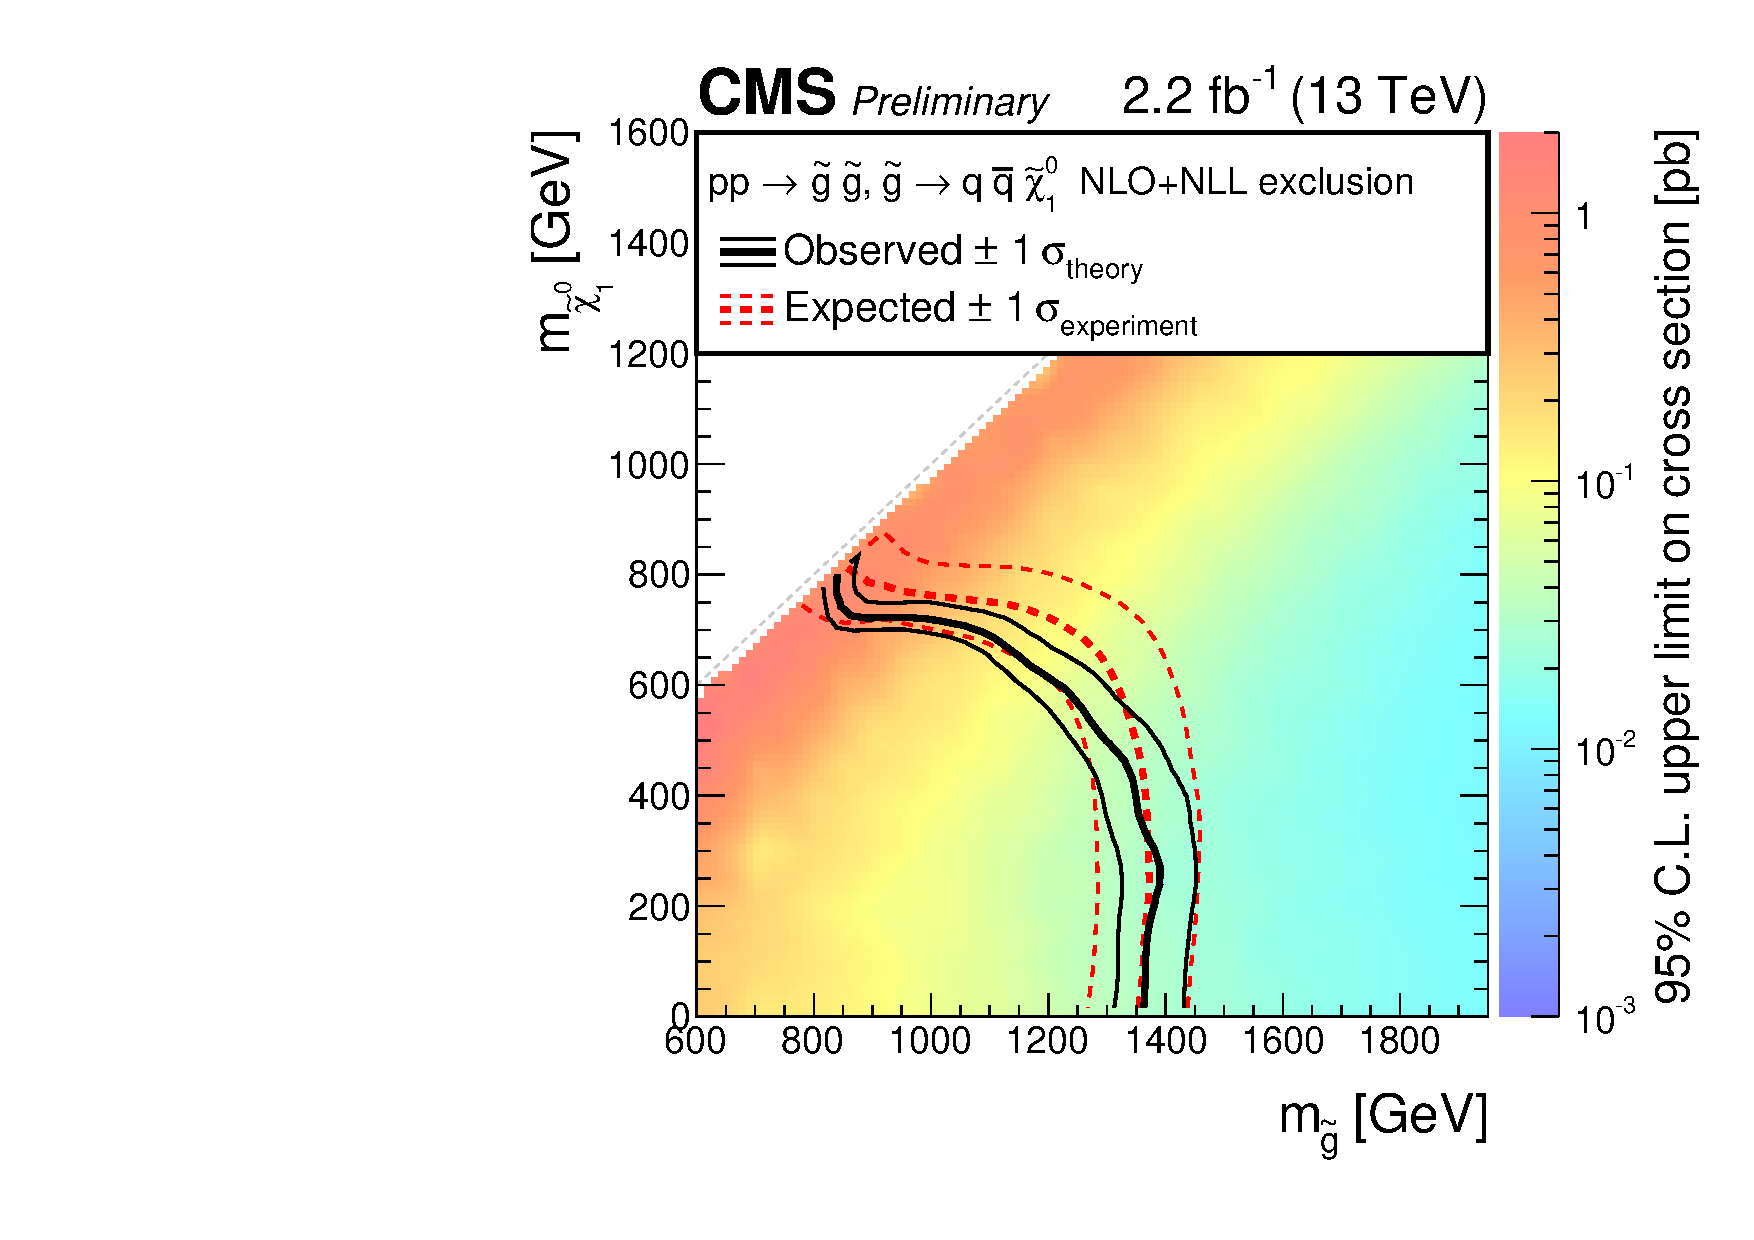
\includegraphics[width=0.65\textwidth]{t1qqqqRA1XSEC.pdf} \\
    \caption{Observed upper limit on the gluino pair-production cross
      section at 95\% CL (indicated by the colour scale) as a function
      of the gluino and $\chiz_{1}$ masses for gluino three-body
      decays to $b\bar{b}\chiz_{1}$ (top) and $q\bar{q}\chiz_{1}$
      (bottom). The black solid thick line indicates the observed mass
      exclusion region, with the thin black lines reflecting the theoretical
      uncertainty in the production cross section. The red thick
      dashed (thin dashed) line indicates the median (${\pm}1 \sigma$
      experimental uncertainty) expected exclusion.
      \label{fig:limits-sms} }
  \end{center}
\end{figure*}

Figure~\ref{fig:limits-sms} shows the observed upper limit on the
production cross section at 95\% confidence level (CL) as a function
of the gluino and LSP masses for a range of simplified models assuming
pair production of gluinos. The observed excluded regions are
determined for gluino pair production assuming decoupled squarks. Also
shown are the observed excluded regions when varying the production
cross section by its theoretical uncertainty, and the expected
excluded region with the ${\pm}1$ standard-deviation ($\sigma$)
variations. The search places stringent limits in the mass parameter
space, with observed exclusions in gluino and LSP masses as high as
$\sim$1550\gev and $\sim$950\gev, respectively.

%%__________________________________________________________________||
